\section{Perception Module}

This is the first block of the proposed system. As it name indicates, it is responsible for apprehend the incoming images (RGB and depth) from the sensor, and generate a significant output to be interpreted by the actuation module. Its structure follows a certain pipeline along the images, which will be described next.


\subsection{Person Detection}

On first place, the incoming RGB images are passed through an \emph{object detection} module. It is powered by a CNN, which has a special architecture designed in \cite{ssd} for this purpose: SSD (\emph{Single-Shot Multibox Detector}). This kind of detection technique stands out by its prediction speed, because \emph{it performs a single feed-forward pass} of the image through the network, unlike the rest of \emph{state-of-the-art} techniques. These other approaches perform successive feed-forward passes through the network, what makes them consequently much slower, as it can be seen on a timing experiment performed during this project, with different detection architectures (Table \ref{tab:model_tests}).\\

\begin{table}[h]
	\centering
	\begin{tabular}{|c|c|c|c|}
		\hline
		\textbf{Architecture} & \textbf{Base network} & \textbf{Dataset} & \textbf{Mean inference time} (ms) \\ \hline
		ResNet  & Inception  & COCO & 820.71 \\ \hline
		SSD  & MobileNet  & COCO & 107.43 \\ \hline
		ResNet  & 101  & COCO & 786.49 \\ \hline
		ResNet  & 50  & COCO & 515.28 \\ \hline
		ResNet  & 101  & COCO & 63.97 \\ \hline
		Faster-RCNN  & ImageNet  & ILSVRC2014 & 703.99 \\ \hline
		Faster-RCNN  & Inception  & COCO & 352.20 \\ \hline
		ResNet  & 50  & COCO & 793.87 \\ \hline
		SSD  & MobileNet  & COCO & 102.85 \\ \hline
		ResNet  & 101  & COCO & 898.59 \\ \hline
		Inception  & ResNet  & OID & 792.42 \\ \hline
		\textbf{SSD Lite}  & \textbf{MobileNet}  & \textbf{COCO} & \textbf{68.13} \\ \hline
		ResNet  & 101  & Kitti & 111.29 \\ \hline
		Inception  & ResNet  & OID & 667.76 \\ \hline
	\end{tabular}
	\caption{Timing performance tests for several detection models. The selected implementation appears in \textbf{boldface}.}
	\label{tab:model_tests}
\end{table}

On this structure, the desired image to input has to be reshaped to 300$\times$300 px, which is a typical shape for this type of CNN architecture. As visualized on Fig. \ref{fig:perception_ssd}, it extracts a set of activation maps on its \emph{base network} o Feature Extractor (\emph{MobileNet}) in the selected network model, and position and class inferences are made later, on multiple image scales. In last place, a \emph{Non Maximum Suppressor} is applied, retaining only the most confident detections, which are adjusted to a correct bounding box shape.\\

\begin{figure}[h]
	\centering
	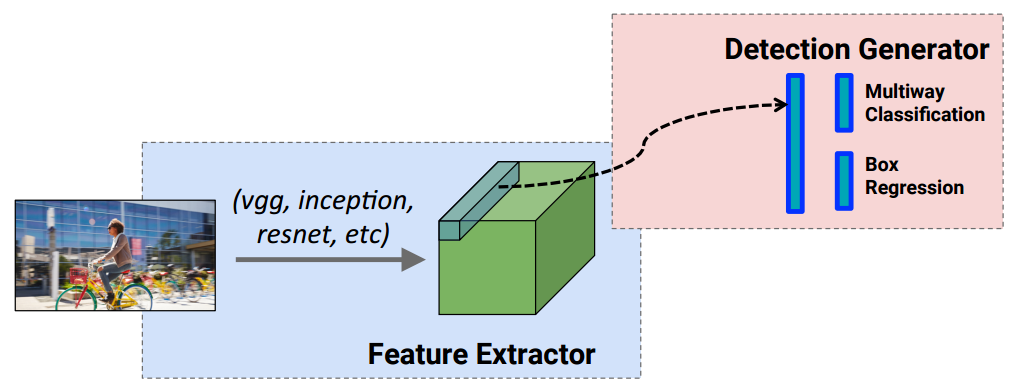
\includegraphics[width=3in]{images/SSD_schematic}
	\caption{Schema of the SSD architecture.}
	\label{fig:perception_ssd}
\end{figure}




This system provides an accurate and efficient object detection, returning for each processed image:

\begin{itemize}
	\item \emph{Classes:} the detected classes (person, cell phone, airplane, dog \dots) inferred for each detected object.
	
	\item \emph{Scores:} the confidence $\in [0,1]$ the network has on each object belonging to the decided class.
	
	\item \emph{Boxes:} the coordinates of the rectangular \emph{bounding box} which wraps the detected object, expressed as the coordinates of two opposite corners of it.
\end{itemize}

Although the used SSD model is capable to detect up to 80 object classes, the proposed system only retains those detection corresponding to \emph{persons}, as it is what we are interested to follow.\\


Hence, this results on a light \emph{person detection}, perfectly capable to work on a real-time operation on a standard level hardware. Our implementation is capable to handle different network models and architectures on a \emph{plug and play} manner, just pointing the model file (in the specific TensorFlow \texttt{.pb} format) to it.



\subsection{Face detection}

Once the existing persons on the image have been detected, the next phase is to search their faces, in order to know whether any of them corresponds to the person to follow. In order to do this, we implement the classical Viola and Jones face detection algorithm (presented on \cite{viola-jones}). This algorithm, which comprises \emph{Haar} features (Fig. \ref{fig:perception_haar}), is a simple algebraic method which takes advantage of the typical illumination pattern of a face (due to its physical shape) to detect promising regions of the input image to contain a face. To test a \emph{Haar} feature on a specific grayscale image, the feature is slided through it, and a simple operation is performed (black pixels subtracted to white ones). If the result is positive along all the feature, the region where it has been applied has passed the test.\\

The image introduced in the system is divided into \emph{regions}, which are passed through a \emph{cascade} of tests, where the non-compliant regions are immediately discarded. The accepted ones pass to a slightly more complex feature each time, and the regions which pass all the features are supposed to contain a face. This progressive region dismiss makes it an efficient algorithm, capable of run simultaneously with the rest of processes. This entire process is performed with an OpenCV\footnote{Open source image processing library.} method.\\

\begin{figure}[h]
	\centering
	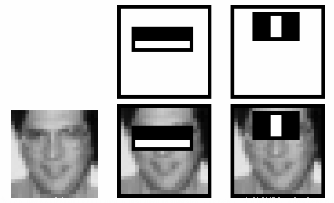
\includegraphics[width=2.5in]{images/haar_on_face}
	\caption{\emph{Haar} features applied on a face.}
	\label{fig:perception_haar}
\end{figure}


As the previous block detected persons inside the image, this face detection algorithm is only applied inside the instance of the detected persons, in order to avoid false positive detections.\\



\subsection{Person and face trackers}

The previously described methods perform respective person and face detections, and although they behave in a robust way, the obtained output can suffer spurious components, due to lighting or occlusive conditions. As this can interfere with the desired following capability, the system palliates the effect of these false positive/negative detections implementing a time-spatial \emph{trackers}, which filter the detection outputs (\emph{candidate detections}). This filter attributes each person/face its coordinates inside the image, and takes into account the number of successive frames that a new response has been detected. If it surpasses a \emph{patience} threshold, it is taken as reliable (\emph{tracked detections}). Otherwise, it is taken as a spurious output. This way, a partial occlusion, which hampers a particular person detection, does not cause the elimination of that person, until it has not been lost for a while. The same happens with void detections which generally happen on a punctual way on a frame.\\

This tracking procedure can be observed in Fig. \ref{fig:perception_tracker}, in the \emph{person detection} case, but it is applied in the same way for \emph{face detection} in the proposed system.\\

\begin{figure}[h]
	\centering
	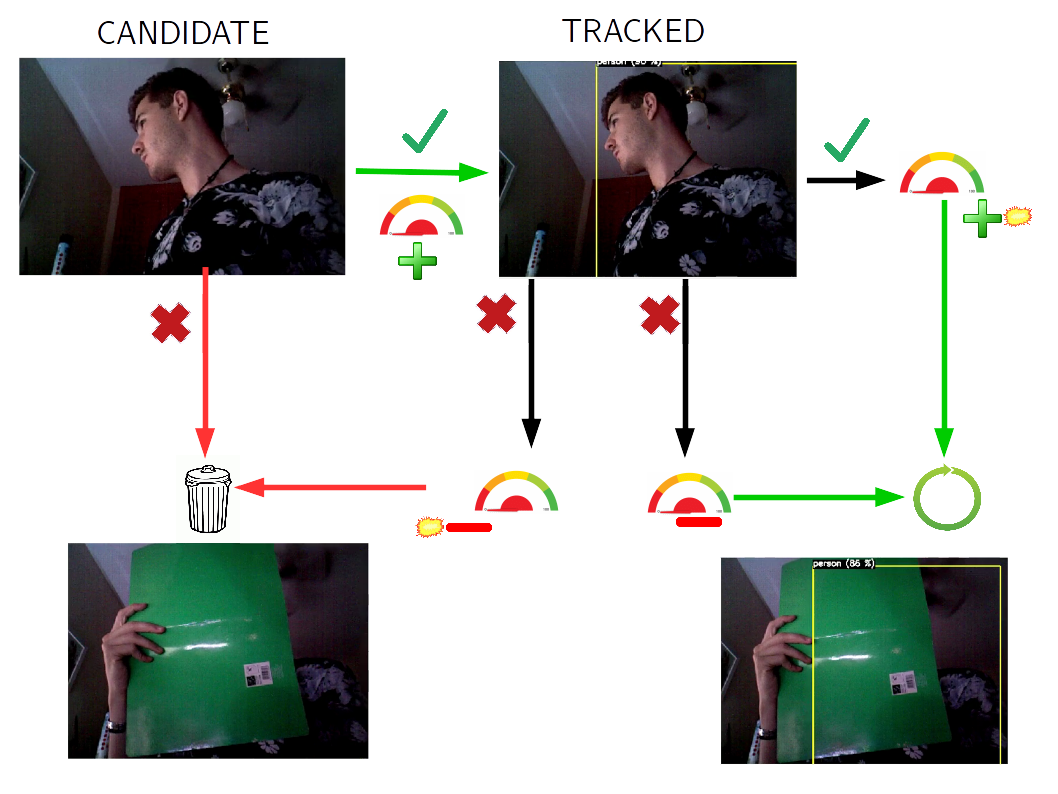
\includegraphics[width=3in]{images/person_tracker}
	\caption{Tracking process for a person detection.}
	\label{fig:perception_tracker}
\end{figure}


\subsection{Face reidentification}

The previous trackers turn the spurious output of the detection systems into tracked and reliable detections. Hence, they can be used to perform \emph{identification} tasks. For this purpose, a parallel CNN, \emph{FaceNet} (presented in \cite{facenet}), is used. This network \emph{maps} a face image, extracting some key features, into a 128-dimensional Euclidean space, where faces are represented by what is called \emph{embeddings} (feature vectors). The Euclidean $L^2$ distance (Eq. \ref{eqn:eucl_distance}) existing between two of this embeddings stands for the \emph{face similarity} between that faces.\\ 

\begin{equation}
d(\vec{f_1}, \vec{f_2}) = \sqrt{\sum_{i=1}^{128}(f_{1_i} - f_{2_i})^2}
\label{eqn:eucl_distance}
\end{equation}

Hence, we can consider that two embeddings belong to the same face if their distance is below a threshold, which has experimentally been set to $1.1$.\\


The proposed solution makes use of this, computing on real time the embeddings of each detected (and tracked) face. Once this has been performed, it compares the similarity between these embeddings and the one corresponding to the target person (computed when the program starts, from a given image of the \emph{person to be followed}). Something to consider is that, to avoid penalties on similarity due to lighting conditions, a previous blurring and \emph{prewhiten} (on Eq. \ref{eqn:perception_normalization}, with $x$ as the color channel, $\mu$ as its mean and $\sigma$ as its standard deviation) are performed on each face inputted on the \emph{FaceNet}.

\begin{equation}
x' = \frac{x - \mu}{\sigma}
\label{eqn:perception_normalization}
\end{equation}

This can be checked in Fig. \ref{fig:perception_tracker} , where it can be observed that the same face in different lighting situations yield embeddings with a distance lower than the threshold.

\begin{figure}[h]
	\centering
	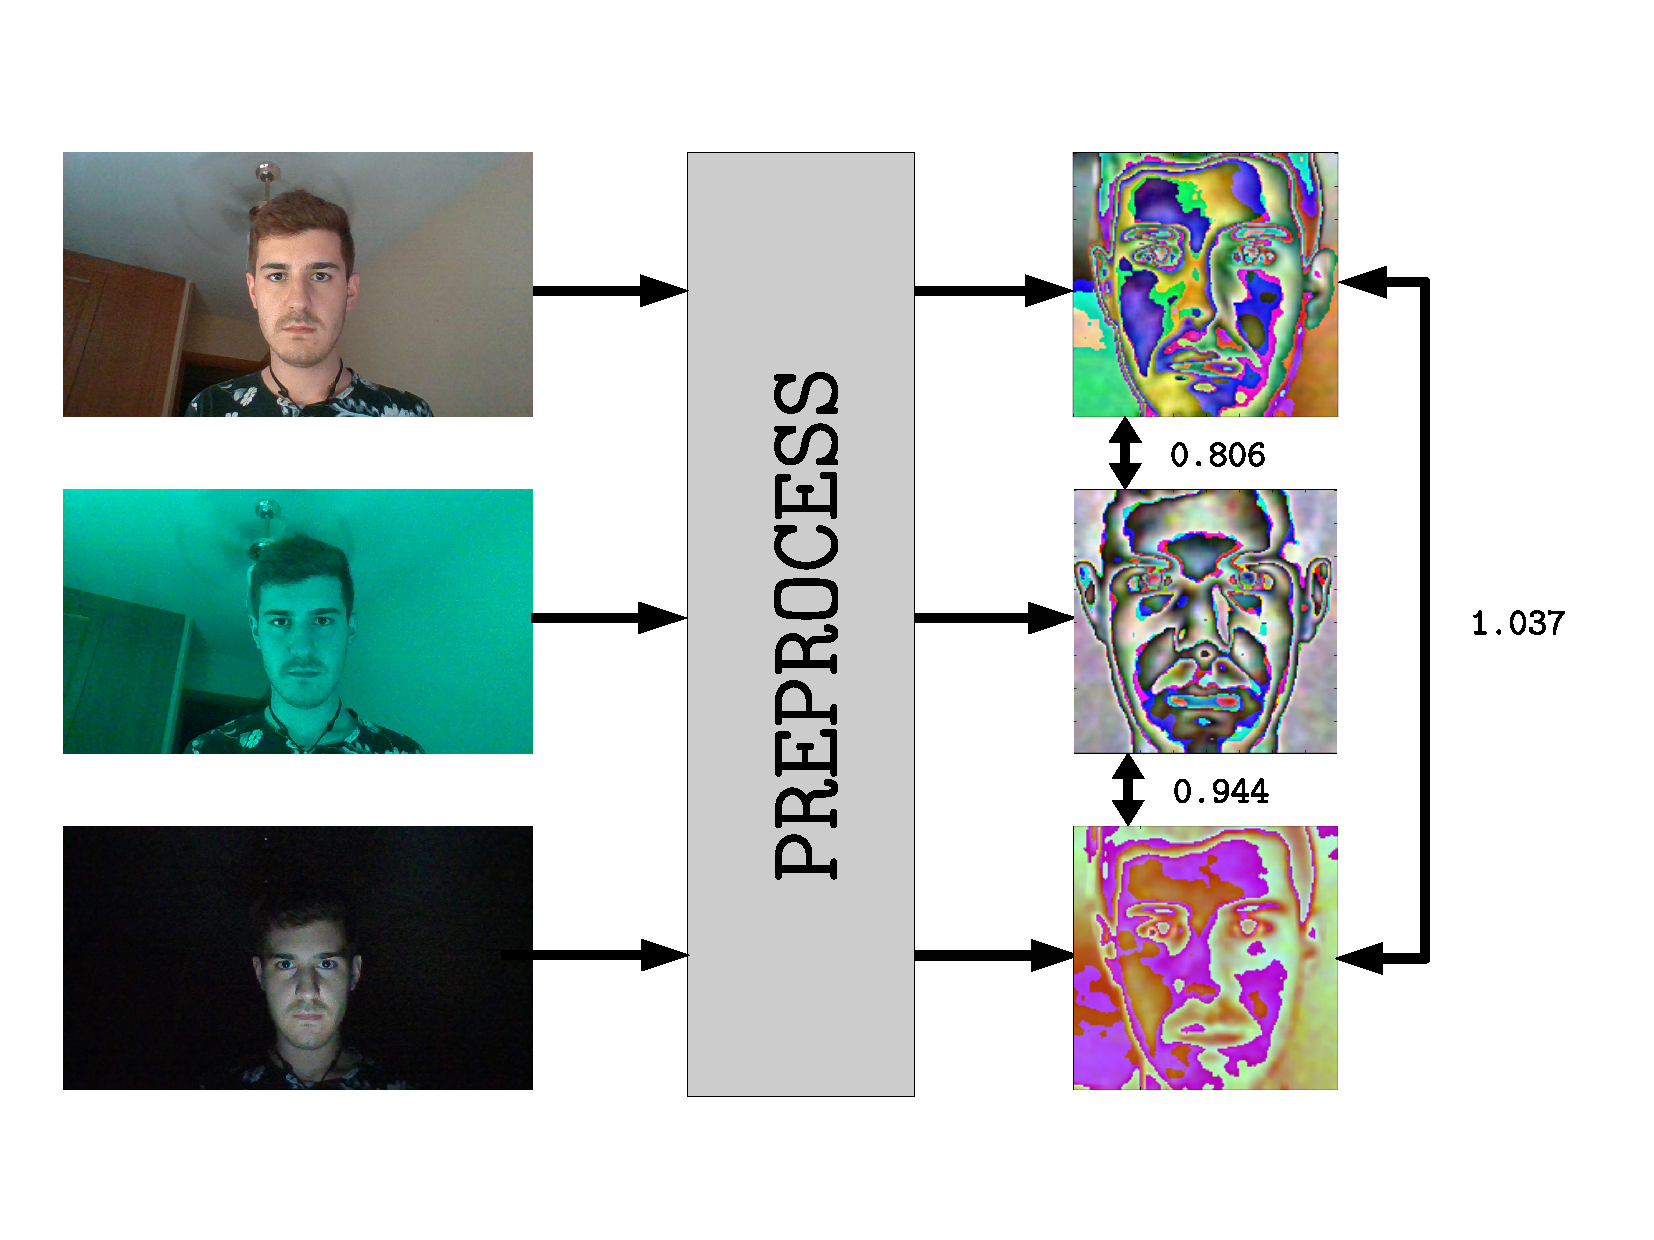
\includegraphics[width=3in]{images/facenet_prewhiten}
	\caption{Relative distances between the same face on different lighting situations. Color patterns on the right images are not representative, as they depend on the numeric range of the plotted image.}
\end{figure}



\vspace{0.4in}

All this described pipeline allows the system to discern if the target person is being seen right now. In addition, it is not necessary to detect its face every time, as the person tracker is capable to infer that a new person detection on a near location to the last position of the target person corresponds to the new location of the tracked person, without needing to see its face.